\documentclass[a4paper]{article}

\usepackage[english]{babel}
\usepackage[utf8]{inputenc}
\usepackage{amsmath}
\usepackage{graphicx}
\usepackage[colorinlistoftodos]{todonotes}

\begin{document}

\begin{titlepage}
	\centering
	

\includegraphics[scale=0.6]{Wits-logo-colour-left-600x300}
	\vspace{1cm}
	
\newcommand{\HRule}{\rule{\linewidth}{0.5mm}} % Defines a new command for the horizontal lines, change thickness here

{\scshape\Large University of Witwatersrand\par}
{\scshape\Large Johannesburg, South Africa\par}
	\vspace{1.0cm}
	{\huge\bfseries Moddeling Competition (SAMMC) \par}
	\vspace{1cm}
	{\Large\itshape Roy Gusinow (1430013)\par}
	\vspace{0.5cm}
	{\Large\itshape Tamlin Love (1438243)\par}
	\vspace{0.5cm}
	{\Large\itshape Omer Elgoni (1391758)\par}
	\vspace{0.5cm}
	{\Large\itshape Leeson Govender (794975)\par}
	\vspace{0.5cm}
	\vfill
	
\HRule \\[0.4cm]
{ \huge \bfseries Stop-Go Traffic}\\[0.4cm] % Title of your document
\HRule \\[1.0cm]
% Bottom of the page
	{\large Semester 1, 2018\par}

\end{titlepage}

\section{Introduction}
\section{Theoretical Background}

\subsection{Clarifications}

We will consider the ordinary situation of road construction on the highway where only one lane may be used. This  begs the question on how to make sure the traffic keeps moving without bias towards one direction. There contains now sharp turns or exits off the road while a car drives along the lane and all cars in the lane must exit before cars off the opposite queue are allowed to go.

Although almost no literature exists on the topic of Stop-Go traffic, much research has been done on other types of traffic flow, including mapping traffic density, $\rho(t)$ of highway congestion as well as waves of oncoming cars. Most importantly, there exists many models which try to optimize 4 way stop intersections. If we consider only two streets allowed that cars are allowed to entered or exit, we find the problem is nearly identical to the Stop-Go problem, as the perpendicular streets of the intersection cannot both have lights at green at the same time. As long as the models we inspect do not include left or right turns in the intersection, the problems are equivalent. The following sections will be based heavily on Michal Kutil's doctoral thesis, \textit{Modelling and Optimization
of Traffic Flow in Urban Areas}.
\subsection{Assumptions and Justifications}

\begin{itemize}
\item \textit{Constant Velocity after 10 meters into lane} - People are cautious in tight lanes and are more likely to adhere to instructions from billboard and traffic engineers. Highways is roughly flat which prohibits changes in speed due to inclines and hills.
\item \textit{Constant distance of 5-10 meters between cars} - Drivers are more cautious when under road construction
\item \textit{Only exits and entrances by the queues is through the stop-go lane} - Drivers cannot make U turns or move out easily on a highway.
\item \textit{The Stop-Go lane flows in only one direction at a time has only a specified number of exits} - There is not enough room for multiple directions or off ramps.
\item 
\end{itemize}

\subsection{Variables}

\begin{itemize}
\item \textit{n} - number of cars in queue, measured in $[n] =$ unit cars (uc)
\item \textit{E} - average waiting time per vehicle, measured in time $[t] =$ time.
\item \textit{S} - total waiting time of all cars
\item \textit{h} - incoming flow rate of cars into the queue, $[h] = uc.s^{-1}$
\item \textit{q} - outgoing flow rate of cars leaving the queue, $[q] = uc.s^{-1}$
\item \textit{v} - average velocity of the car, $[v] =m.s^{-1}$ 
\item \textit{L} - length of the road $[L] = $ m
\item \textit{T} - waiting time, $[T] = s$
\end{itemize}

\subsection{Queue Model}

We start with building a \textbf{queue model} that recreates simple accumulation of vehicles on a street. There are two primary variables which are essential to optimizing this system:

\begin{itemize}
\item \textit{n} - the number of cars in a particular queue, measured in $[n] =$ unit cars (uc).
\item \textit{E} - the average waiting time per vehicle, measured in time $[t] =$ time.
\end{itemize}

We also note that \textit{E} is related to \textit{n} by $E = \frac{S}{n}$, with \textit{S} being the total waiting of all cars in the system. It will become later that it is necessary to continue this solution via a \textbf{discrete form}, as the traffic flow is not continuous i.e we cannot let 1.27 unit cars into the road. More apparent is the abrupt changes of car outflow rates from the changing of the sign from \textit{go} to \textit{stop}, thereby we will present the problem as a system of difference equations.
We now consider two rates, incoming car rate, \textit{h} which represents the amount of cars which enter the queue by driving up the road to join the street. And outgoing car rate, \textit{q} , whereby the cars in front drive off to leave the queue. 

Modelled as a \textbf{differential equation},

\[\frac{dn}{dt} =  h - q\]

\begin{figure}
\centering
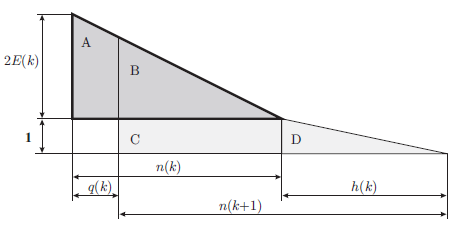
\includegraphics[scale=1]{geo.png}
\caption{Kutil's Geometric Interpretation}
\end{figure}
As a \textbf{difference equation}, Kutil offers a geometric interpretation of triangle pictured in Figure . The bold triangle represents total waiting time $S = E \cdot n$ at initial time k. It has a height of double the average waiting time, a fair assumption for the longest waiting time. It's base is the queue length, n. To move from k to k+1, a new area is formed by increasing the height by 1 unit, decreasing the length by \textit{q(k)} and increasing by \textit{h(k)}. 

In other words, this new area is equivalent to the amount of cars still left in the queue after the front cars are allowed to go, B. All cars increase their waiting time by one unit, encapsulated by area C while the new cars from incoming traffic, \textit{h(k)} is represented by triangle D. 

\[A_B = \frac{E(k) [n(k)-q(k)]^2}{n(k)}\]
\[A_C = n(k) -q(k)\]
\[A_D = \frac{h(k)}{2}\]


All three of these areas together represent the total future waiting time at $S(k+1)$. Thus, we have 
\begin{equation}
S(k+1) = E(k+1) \cdot n(k+1) = \frac{E(k) [n(k)-q(k)]^2}{n(k)} + n(k) -q(k)+ \frac{h(k)}{2}
\label{tot}
\end{equation}
The amount of future cars that we have in the queue must be the sum of the current cars and the incoming/outgoing rate. Thus,
\begin{equation}
n(k+1) = n(k) +h (k) -q(k)
\label{car}
\end{equation}
and therefore we may solve Equation \ref{tot},
\[E(k+1) = \frac{\frac{E(k) [n(k)-q(k)]^2}{n(k)} + n(k) -q(k)+ \frac{h(k)}{2}}{n(k+1)}\]
\begin{equation}
\implies E(k+1) = \frac{\frac{E(k) [n(k)-q(k)]^2}{n(k)} + n(k) -q(k)+ \frac{h(k)}{2}}{n(k) +h (k) -q(k))} 
\label{wait}
\end{equation}

Our denominators indicate that $n(k)>0$ and $n(k) > q(k) - h(k)$. This tells us two things: there must always be cars in the queue and more cars should enter the road than leave, in case it violates the second inequality.
\subsubsection{Equilibrium Points}
Equilibrium points are found by taking Equation \ref{car} and equating the $n(k)$, thus
\[n(k+1) = n(k) = n(k) +h (k) -q(k) \implies h^*(k) = q^*(k)\]
Similarly for the waiting time, Equation \ref{wait} is equated to $E(k)$ and
\[\implies 2E^*(k) = \frac{n^*(k)}{q^*(k)}\]

\subsection{Stop-Go Model}

\begin{figure}[h]
\centering
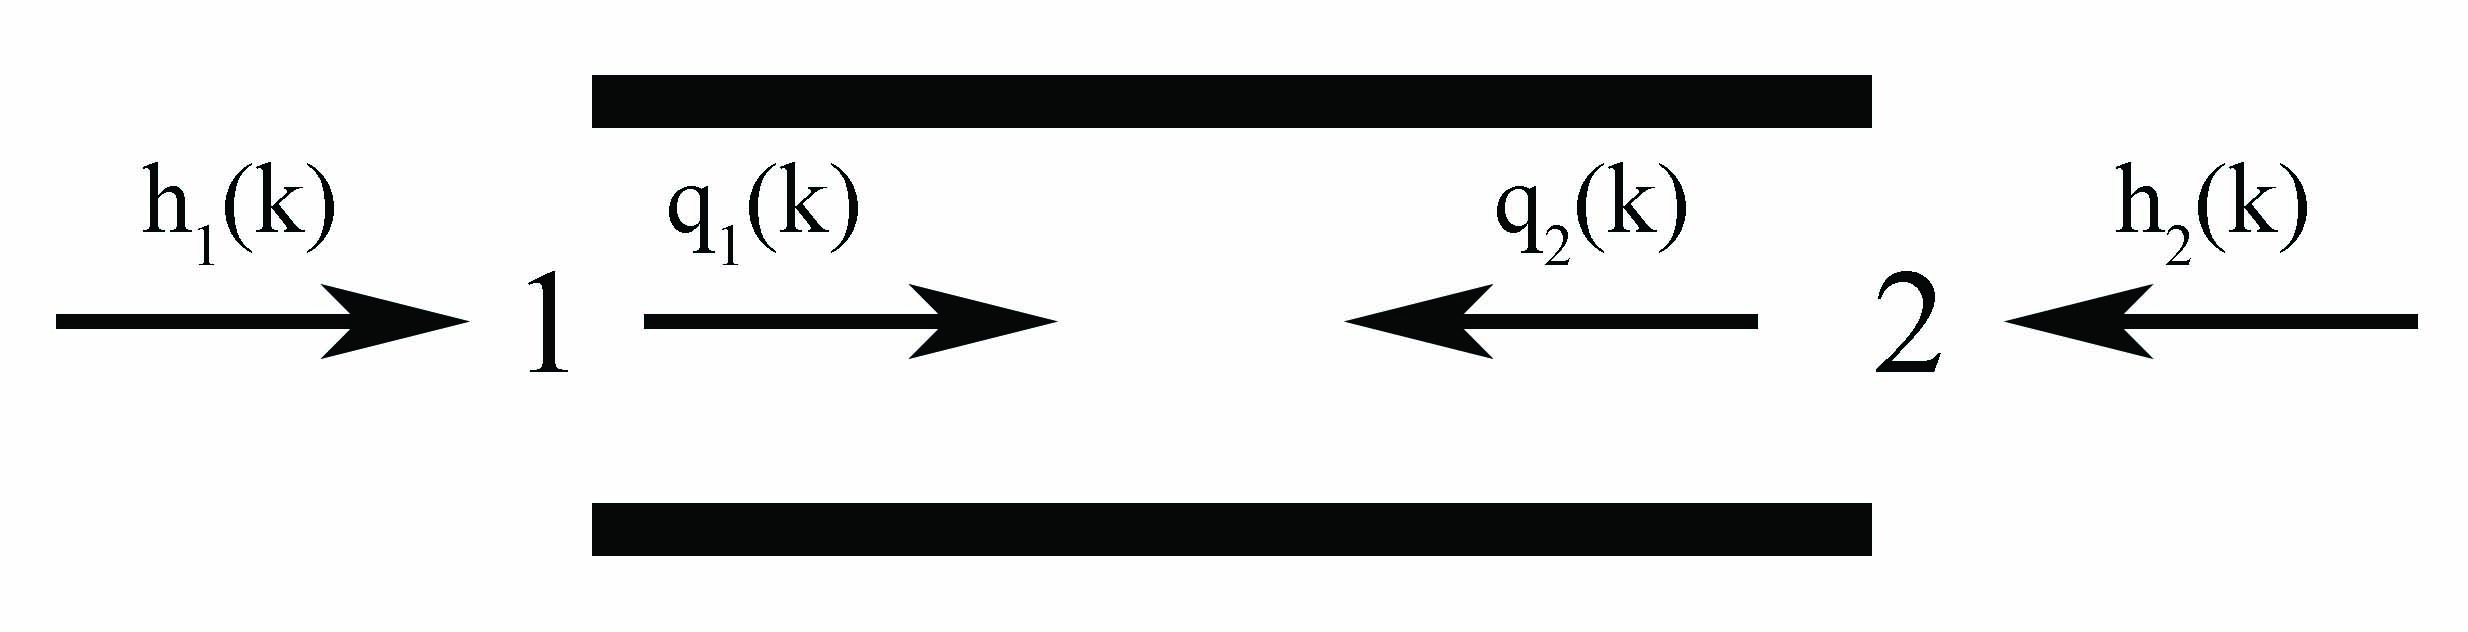
\includegraphics[scale=0.5]{stop.jpg}
\end{figure}
We now consider the Stop-Go model which can simply be considered a queue model with two different, near independent streets. Thus, regions 1 and 2 have different respective numbers of cars in the queue, $n$, average waiting time, $E$ and different incoming/outgoing rates, $h(k)$ and $q(k)$. We define a vector $\bar{x}(k) = (n_1(k), E_1(k), n_2(k), E_2(k))^T$ and write a linearised vector model as,

\[
\begin{pmatrix}
n_1 (k+1) \\
E_1 (k+1) \\
n_2 (k+1) \\
E_2 (k+1) \\
\end{pmatrix}
= \textbf{A} \begin{pmatrix}
n_1 (k) \\
E_1 (k) \\
n_2 (k) \\
E_2 (k) \\
\end{pmatrix}
+\textbf{B} \begin{pmatrix}
q_1 (k) \\
q_2 (k) \\
\end{pmatrix}
+\textbf{C} \begin{pmatrix}
h_1 (k) \\
h_2 (k) \\
\end{pmatrix}
\]
Or, written more succinctly as 
\begin{equation}
\bar{x} (k+1) = \textbf{A}\bar{x}(k) +\textbf{B}\bar{q} +\textbf{C}\bar{h}(k)
\label{num}
\end{equation}
The matrices, \textbf{A}, \textbf{B}, \textbf{C} are determined by the parameters in place. The goal of our model is to minimize delay time amongst the disgruntled drivers. This means that within a certain time period, $C$, there is an optimal time where traffic switches from one direction to another (stop and go). This is called the \textit{switching time}, denoted $\tau_s$. Now, from the time that region 1's gate is closed - $\tau_{s1}$, the last car from this region leaving must still be given time to traverse the lane with length L, with average velocity v. Thus, the time taken for him to reach the other side of the lane is $t = \frac{L}{v}$ and only the will region 2's gate be open - $\tau_{s2}$. We remind ourselves as well that the outgoing rate $q_i (k)$ is only greater than zero when the \textit{i}-th direction/region of traffic is able to go, otherwise it is equal to zero (stop). Combining these concepts yields an updated outgoing rate,
\[\bar{q}(k) = \begin{cases}
(q_1 , 0)^T & k\in (iC, iC+\tau_{s1}) \\
(0,0) ^T & k \in (iC+\tau_{s1}, iC+\tau_{s1} + \frac{L}{v}) \\
(0, q_2)^T & k \in (iC+\tau_{s1} + \frac{L}{v}, iC+\tau_{s1} + \tau_{s2} + \frac{L}{v} \\
(0,0)^T  & k \in (iC+\tau_{s1} + \tau_{s2} + \frac{L}{v}, iC+\tau_{s1} + \tau_{s2} + 2\frac{L}{v})
\end{cases}
\]
where i = 0,1,2... counts the cycle time.

\subsubsection{Minimization}

Our goal now becomes
\[minimize \quad J\]

$J$ is a cost objective function which can be chosen according to how we seek to solve the problem depending on what we would actually like to minimize. Here are possible options:
\begin{itemize}
\item Minimize the difference between the average wait time of cars in regions 1 and 2,
 \[J_1 = \sum_k (E_1(k) - E_2(k))^2\]
 
\item Minimize the average car length over all the queues,
\[J_2 = \frac{1}{T} \sum_k n_1(k)+n_2 (k)\]

\item Minimize the average waiting time over all the queues
\[J_3 = \frac{1}{T}\sum_k E_1(k)+E_2(k)\]
\end{itemize}

\subsubsection{Switching Time}

In each cycle we only allow a certain number of cars to go from each queue to go. While these cars are travelling on the road the road is closed for each side leaving the time we can open the road to be equal to $T -\frac{2L}{v}$.

In this time we must allow both queues to flow for some time. In order to equalize the queues we give each of them time proportional to their size as governed by the equation,
\begin{equation}
T_0 \frac{n_1}{n_1 +n_2}
\end{equation}

so the switching times are as follows:
\begin{itemize}
\item Gate 1 is opened at $t = 0$ and closed at $t = T_0\frac{n_1}{n_1 + n_2}$,
\item Then the cars are allowed to travel to the other side,
\item Gate 2 is opened at 
\[\tau_{sw} = \frac{L}{v} + T_0\frac{n_1}{n_1 + n_2}\]
and closed at t = $\frac{L}{v} + T_0$
\end{itemize}

\section{Experimental Set-Up and Testing}

The model was created in such a way to utilise variables that we can reliably measure and control in an environment like a Stop-Go street on a highway. Although we cannot direct indicate the exact speed and acceleration of cars that pull off when the Go-sign is initiated, and therefore the outgoing rate, \textit{q}, we may control the average rate, by putting small bumpers on the road and fining drivers for either moving too fast or slow. This gives us a general upper and lower bound as well average rate for \textit{q(k)}. With a recommended $80 km.h^{-1}$ and leeway of $20 km.h^{-1}$, we have,
\[v(k) = 80\pm 20 km.h^{-1}\]
We cannot control the incoming rate, \textit{h(k)}, and thus take an mean of previous data. Thus, $h = 0.028 $ according to Kutil's data on the streets of Prague.

We now explain pragmatically how the Stop-Go system will actually work. Infra-red sensors are set up at Regions 1 and 2 just before the cars enter the single lane. This can experimental retrieve current rate of cars \textit{q(k)}. We also set up the sensors every 50 meters stretching up the road from the lane in order to approximately measure the current amount of cars in the queue, $n(k)$ since in traffic with average car length being 4.8 meters and length between cars of 1-2 meters, we may estimate the amount of cars in a stretch of 50 meters being $9\pm$. For example, if the light senses a vehicle at 150 meters but not at 200 meters - we may calculate that the mean amount of cars should be $\frac{9\pm 1}{2} \approx 4 \pm 0.5$ cars. If there is no movement sensed by the light sensor , we can also gather the total waiting time across all cars, \textit{S}, thereby retrieving average waiting time, $E = \frac{S}{n}$. 

Thus, this set-up allows us to monitor to initialize our values for the difference equation, ($E(0), n(0), q(0), h(0)$) and predict what the optimal switching time should be based on our cost function, \textit{J}. Clearly, if our model works, the data from the infra-red sensors will correspond to predictions made by the system of difference equations. However, due to errors present in the measurements as well as several assumptions that are being made. We will have uncertainty in our expected values. Demonstrated below utilizes Equation (\ref{car}) to show how errors grow iteratively.
\[n(k+1) \pm \Delta n(k+1)= n(k)\pm \Delta n(k) +h (k)\pm\Delta h(k) -q(k)\pm\Delta q(k)\]
\[\implies \Delta n(k+1) = \Delta n(k) + \Delta h(k)+ \Delta q(k)\]
\[\implies \Delta n(k+2) = \Delta n(k+1) + \Delta h(k)+ \Delta q(k) \]
\[= \Delta n(k) + \Delta h(k)+ \Delta q(k) + \Delta h(k)+ \Delta q(k) = 2\Delta n(k) + 2\Delta h(k)+ 2\Delta q(k)\]

Thus, the error in number of cars in the queue increases linearly. To restrict this, we replace the calculated value with experimental value, thereby ensuring the only error present is one associated with measurement and estimation presents, something which can always be improved with more funding and technology. 

We see that response system of a network of infra-red sensors connected to a signal a dedicated device such as a laptop will compute the switching time for each time cycle, C and update its data at the end of each cycle and compute a new switching time. The traffic controllers sitting at both regions 1 and 2 will communicate to ensure it is safe to open and close gates accordingly via radio transceivers. It is important to note since the computations is only needed for the next cycle time, a device as simple as a smart phone has enough CPU power necessary to estimate the switching time, given a reasonably large step size in k.
\section{Results and Discussion}
Equation (2) has the solution:
\begin{equation}
n(k)=n(0)+k(h-q)
\end{equation}
assuming $h$ and $q$ are constant. We can extend this solution to include the piecewise $\bar{q}(k)$ presented in section 2.5. When plotting this difference equation for each queue over a single cycle, we obtain the following graph.
\begin{figure}[h]
\centering
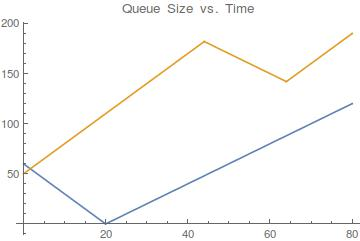
\includegraphics[scale=0.5]{QueueSizeGrowth.jpg}
\end{figure}
This particular figure was obtained using the following parameters:
\begin{itemize}
\item $h_{1}=2$ cars/unit time
\item $q_{1}=5$ cars/unit time 
\item $n_{1}(0)=60$ cars
\item $h_{2}=3$ cars/unit time
\item $q_{2}=5$ cars/unit time
\item $n_{2}(0)=50$ cars
\item $\tau_{sw1}=20$ units of time
\item $\tau_{sw2}=20$ units of time
\item $\frac{L}{V}=25$ units of time
\end{itemize}
As can be seen above, the size of Queue 1 decreases linearly (provided $q_{1} > h_{1}$) when traffic is flowing (from time 0 to $T_{sw1}$), and increases linearly when traffic is stopped (from time $T_{sw1}$ to the end of the cycle). The size of Queue 2 can behaves differently across three periods of time. From time 0 to $\tau_{sw1}+\frac{L}{V}$, traffic is not flowing and thus the queue grows linearly. From time $\tau_{sw1}+\frac{L}{V}$ to $\tau_{sw1}+\tau_{sw2}+\frac{L}{V}$, traffic is flowing from queue 2 and thus the queue size decreases (provided more cars are let through than arrive). Finally, from time $\tau_{sw1}+\tau_{sw2}+\frac{L}{V}$ to the end of the cycle ($\tau_{sw1}+\tau_{sw2}+2\frac{L}{V}$), traffic has stopped flowing as the cars from queue 2 travel through the road.

From these results, we can conclude that in order to keep the queue sizes from growing overly large, switching times should be sufficiently large and proportional to queue size. This supports our conclusion in section 2.5.2. A smaller $\frac{L}{V}$ value ameliorates the situation and thus car speed through the road should be kept as high as is safe.

For a single side of the road, we can also investigate how  Equation (3) (the average waiting time) evolves over time (this discards the piecewise $\bar{q}(k)$ used above for a constant $q$).

For $q < h$, we obtain the following graph:
\begin{figure}[h]
\centering
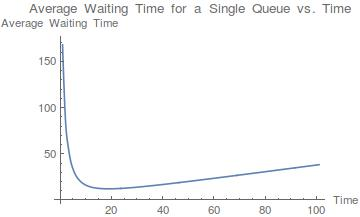
\includegraphics[scale=0.5]{WTQLH.jpg}
\end{figure}
Here it can be seen that waiting time grows large as time progresses. This is certainly not ideal.

For $h \leq q$, we obtain the following graph:
\begin{figure}[h]
\centering
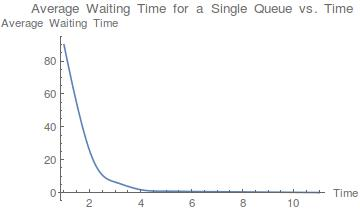
\includegraphics[scale=0.5]{WTHLQ.jpg}
\end{figure}
Here waiting time tends assymptotically to 0. This is certainly ideal and further supports our conclusion that outgoing traffic must exceed incoming traffic. 

Obviously this is a huge simplification of the model, but it is useful nevertheless for the purposes of investigating how average waiting time grows over time.
\section{Extensions}

\subsection{Multiple Stop-Go System}

The model we create for a single Stop-Go system is easily scalable and modular in nature. For a multiple stop go system, we simply relate the outgoing rate of flow of cars, \textit{q(k)} to the next incoming stop-go point where its incoming rate is \textit{h(k)}. Thus, from point 1 to point 2, clearly we have
\[q_1 (k) = h_2 (k)\]

To clarify, the first stop-go point now has stable incoming flow rate, \textit{a(k)} and the last stop-go point has regulated outgoing flow rate, \textit{b(k)} now, ever intermittent flow is now related to each other by the above equation.

\subsection{3 Way Stop-Go System}

As stated previously, our model is not just extendible in the addition of multiple stops, but also scalable for the addition of multiple roads and exits. The dimensions of the system of our equations increases by one so Equation (\ref{num}) becomes
\begin{equation}
\bar{x} (k+1) = \textbf{A}\bar{x}(k) +\textbf{B}\bar{q} +\textbf{C}\bar{h}(k)
\end{equation}

with 
\[\bar{x}  = 
\begin{pmatrix}
n_1 (k) \\
E_1 (k) \\
n_2 (k) \\
E_2 (k) \\
n_3 (k) \\
E_3 (k) \\
\end{pmatrix} \qquad \bar{q} = 
\begin{pmatrix}
q_1 (k) \\
q_2 (k) \\
q_3 (k) \\
\end{pmatrix} \qquad \bar{h} = 
\begin{pmatrix}
h_1 (k) \\
h_2 (k) \\
h_3 (k) \\
\end{pmatrix}
\]

We expand our out flowing system to now include the three switching times. We will also forgo our calculation of how long it takes a car to move drive from one region to another, instead simply referring to this time as $T_i$. Thus, a complete cycle can again be represented by,

\[\bar{q}(k) = \begin{cases}
(q_1 , 0, 0)^T & k\in (iC, iC+\tau_{s1}) \\
(0,0,0) ^T & k \in (iC+\tau_{s1}, iC+\tau_{s1} + T \\
(0, q_2, 0)^T & k \in (iC+\tau_{s1} + \frac{L}{v}, iC+\tau_{s1} + \tau_{s2} +T_1 \\
(0,0, 0)^T  & k \in (iC+\tau_{s1} + \tau_{s2} + T_1, iC+\tau_{s1} + \tau_{s2} + T_1 +T_2) \\
(0,0, q_3)^T  & k \in (iC+\tau_{s1} + \tau_{s2} + T_1 +T_2, iC+\tau_{s1} + \tau_{s2} + T_1 +T_2) \\
(0,0,0) ^T & k \in ( iC+\tau_{s1} + \tau_{s2} + T_1 +T_2,  iC+\tau_{s1} + \tau_{s2} +\tau_3 + T_1 +T_2)) \\
\end{cases}
\]


\section{Conclusions}
Clearly many of the models presented above are not easily solvable. Numerical techniques are required to obtain ideal values for switching times. However, Equation (5) presents us with a simple, computationally inexpensive method to calculate switching times. While not completely taking into account the complicated dynamics of the system, it is nevertheless robust and practical.
\subsection{Advantages and Disadvantages}
Our strategy has the following advantages:
\begin{itemize}
\item The infrared technology will accurately account for the number of cars in the queue at any given time.
\item We can track when the last car of a given period has travelled the entire distance of the stop-go before instructing the opposite direction to flow. This will avoid head-on collisions
\item Our dynamic models constantly computes new data (rate of incoming and outgoing traffic) and thus improves efficiency of traffic flow with each cycle.
\item Our speed restrictions ensure that we can more accurately predict the speed at which drivers move which enhances the accuracy of our model and in turn the efficiency of traffic flow. A second and more important result of our speed restrictions is that it will ensure drivers safety and reduces road rage.
\end{itemize}
Our strategy does, however, have some disadvantages:
\begin{itemize}
\item By capturing the average velocity and time of each car we cannot accurately depict how each car will accelerate and wait to cover the allocated distance of the stop-go
\item Infrared sensors may break or malfunction due to poor weather conditions
\item Sensor technology is expensive
\end{itemize}

\section{References}

\subsection{Websites}


\subsection{Textbooks}


\end{document}



